\documentclass[sigconf]{acmart}

\usepackage{hyperref}

%\usepackage{endfloat}
%\renewcommand{\efloatseparator}{\mbox{}} % no new page between figures

\usepackage{booktabs} % For formal tables

\settopmatter{printacmref=false} % Removes citation information below abstract
\renewcommand\footnotetextcopyrightpermission[1]{} % removes footnote with conference information in first column
\pagestyle{plain} % removes running headers


\begin{document}
\title{Big Data and Sentiment Analysis}
\author{Syam Sundar Herle}
\orcid{HID219}
\affiliation{%
  \institution{Indiana University}
  \streetaddress{711 N Park Ave}
  \city{Bloomington} 
  \state{Indiana} 
  \postcode{47408}
}
\email{syampara@iu.edu}

\begin{abstract}
Opinion mining is an art of extracting opinions of author, speaker or writer from their written text or spoken words, opinion mining is done by employing Natural Language Processing ,text analysis, Artificial Intelligence. This paper shows where the Big Data meets Sentiment Analysis and the issues related in using Big Data in Sentiment Analysis. How the consumer needs and product evaluation is done while using Big Data in opinion mining. 
\end{abstract}

\keywords{Big Data, i523, hid219, Opinion Mining, Natural Language Processing, Artificial Intelligence, Sentiment Analysis}

\maketitle
\section{Introduction}

Usually the sentiment analysis can be defined as classifying a piece of written text into positive,negative or neutral state. This is also known as opinion analysis as it derives the opinion of the author. Said that, now a days, user's and consumers write reviews, opinions on online for a product or service given to them. The growth of web and internet has enabled user or consumers to communicate among each other and write up more reviews about products and has made the web more subjective and opinionated. As a result, huge amount of data in the form of texts are available from online which are rich in information, which are users review and opinion about products and service delivered to them. Which in turn can be used by the product owners to meet the consumer needs and demands, and provide quality products and identify the issues in products and much more. Unbiased and independent reviews about a product are the main decision making entity usually used by peoples while purchasing a product. 
Opinion mining is usually employed for the knowledge retrieval from textual contents such as review and comments. Opinion mining results the the textual content in one of the three categories namely positive, negative and neutral. Positive opinion are good in yielding good financial gains and fame and good business for product owners. On the other hand negative reviews helps in identifying the issues of the products, having said that some people usually write fake reviews to boost their financial gain or discredit their competitive product. These type of reviews are known as opinion spammers.
\section{Sentiment Analysis}
As defined earlier, sentiment analysis or opinion mining is the study of peoples opinion, attitude and emotion towards a product or any other entity. Usually the sentiment analysis is done on the textual contents like reviews of product, twitter tweets and comments in public blog about any entities. The overview of the sentiment analysis can be seen the Figure \ref{f:SA}.

\begin{figure}[!ht]
  \centering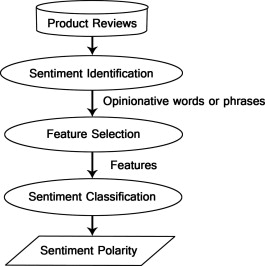
\includegraphics[width=\columnwidth]{images/sa.jpg}
  \caption{Sentiment Analysis on product review \cite{sentianalysis}}\label{f:SA}
\end{figure}

Overall, sentiment analysis is considered to be a classification process, which is done by three different types, the first one is being document sentiment analysis where the texts of documents are used to classify the opinion of the whole documents, the other type is sentence sentiment analysis where the texts of the sentence is used to classify the opinion of the sentence and third one is being aspect-level sentiment analysis where sentence or document are classified with respect to specific aspects of entity (product or service). 
\subsection{Data}
In the first step of Sentiment Analysis, data are collected from online, the preferred data are reviews of product as these data are textual contents and unstructured and rich in information. These data are important in the sentiment analysis as the business owner can make use of the analysis of these data (review of product) to learn about users opinion about the product. The social media network are one of the good and important source of these types of data as users and consumers interact and post review of the products from their own accounts. 

The second important step is identifying the words or phrases which are useful in the forming the opinion in the sentence or document based on the type of sentiment analysis we intend to do as told in earlier paragraph. The following sub-section describes the next each steps in sentiment analysis in detail.

\subsection{Feature Selection}
The very important step in sentiment analysis is extracting features needed for the analysis, some of the feature selection used are,\textbf{Bag of Words and Frequency} in which a vector of binary is used as features, the binary vector comprises of 1 and 0 based on the presence of words in the document or sentence and forming a bag of binary vector for all words. The other weight used in these type of feature is the frequency of the words in the sentence or document. 

The next type of features used in sentiment analysis is \textbf{Part Of Speech} where the part of speech tagger is used to create features, in this method grammatical context tag of the words in sentence or document is used, these types features helps to find the emotion of the author from his or her texts.

The other features employed are \textbf{Opinion words and Negations} where features are built based upon the words which determines the words as bad or good and negation features gives overall appearance of the negative words in sentence or document.
\subsubsection{Feature Selection Methods} 
Here we can see some of the methods employed to extract and select features to perform sentiment analysis on the sentence or document. Usually feature selection can be done by two types of methods, \textbf{Lexicon-based} \cite{lexi} method and \textbf{Statistical-based} \cite{statis} method. The first method needs human annotation like bag of words (BOW) \cite{lexi} but the second method is usually is fully automated. Some of the statistical methods used in feature selection are given as follows,
\subsubsection*{Chi-Square $\tilde{\chi}^2$} : In chi-square test, the correlation between the term and categories is checked. According to \cite{sentianalysis} Consider n documents in any collection, and $p_{i}(w)$ be the conditional probability of class $i$ for document which contains the word $w$. and $P_{i}$ be the global fraction of document containing the class $i$, and $F(w)$ be the global fraction of document containing the word $w$. So the chi-square can be calculated as given in \cite{sentianalysis},
$$\tilde{\chi}^2 = \frac{n.F(w)^{2}.(p_{i}(w)-P_{i})^2}{F(w).(1-F(w)).P_{i}.(1-P_{i})}$$

The chi-square gives weights value for the words in the document and these value can be used as features for the sentiment analysis.

\subsubsection*{Information Gain} : In this method features are created based on the ranks of Information Gain entropy grouped in descending order. "The information gain usually measures the amount of information in bits about the class prediction, it also measures the expected reduction in entropy" \cite{Duch2006}.

\subsubsection*{Point-Wise Mutual Information} : This model provides mutual information between feature and classes, and this is derived from the information theory. According to \cite{sentianalysis} the point-wise mutual information, $M_i(w)$ is the information between the word $w$ and class $i$. So, we in laymen terms , the 
PMI \cite{sentianalysis} is the ratio between expected co-occurrence of class $i$ and $w$ which is given by $F(w).p_i(w)$ and the true occurrence which is given by $F(w).P_i$, so the PMI is defined as,
$$M_i(w) = log\bigg(\frac{F(w).P_i}{F(w).p_i(w)}\bigg)$$

The word $w$ is positive correlated to class $i$ if the value of $M_i(w)$ is greater than 0. Comparing with chi-square, PMI is not normalized value and hence for most of the feature selection chi-square is used.

\subsection{Classification Technique}

The classification technique employed for the sentiment analysis can be done by three approaches, Machine Learning approach, Lexicon based approach and use of both ML and Lexicon approach. In this sub-section we will walk through some of the techniques followed in all the three approaches.

\subsubsection{Machine Learning Approach}
Typical machine learning algorithms or predictive models are used in this approach, typically the ML approach can be divided into two models, Supervised learning and Unsupervised learning. 
\subsubsection*{Supervised Learning} : In supervised learning, a model is trained with the help of the labeled training data set and evaluated on the unseen data set which are known as test data set. After evaluating the test data classification accuracy are calculated to know how good the trained model is in classifying. Some of the supervised learning model used in sentiment analysis for classification techniques are,
\begin{itemize}
    \item Naive Bayes classifier : The Naive-Bayes is one of the probabilistic classifier, which works based on probabilities value to determine class. According to \cite{sentianalysis} the Naive-Bayes model predicts the posterior probability of a class to which the document belongs to, based on distribution of words in the document. For a given features it calculates the probability of the label assuming all the features $(f_i-f_n)$ are independent to each other, the Naive-Bayes follows the following equation to classify the class to which the document belongs to given the features, the features are generated by the Bag Of Words model.
    \begin{equation*}
        P(label/features) = \frac{P(label)*P(f_{1}/label)*.*P(f_{n}/label)}{P(features)}
    \end{equation*}
    As the above equation assumes the naive assumption of independence and uses Bayes theorem, it is known as the Naive-Bayes model.
    
    \item Support Vector Machine : Support Vector Machine model works based on the linear separation of the features which separates features in the search space to separate them based upon their classes, SVM is one of the linear classifier used in supervised learning ML approach. In SVM, the features are transformed to a higher dimensional state space and hyperplanes are used to separate the features, hyperplanes are determined by support vectors, which are features closer to the decision boundary of the separation of the features. For $n$ class of class the model needs $n-1$ support vectors. "SVM can construct a nonlinear decision surface in the original feature space by mapping the data instances non-linearly to an inner product space where the classes can be separated linearly with a hyperplane" \cite{sentianalysis}. In the case opinion mining, the classification are two positive and negative and hence one support vector is needed to do sentiment analysis.
    
    \item Neural Network : Neural Network (NN) consists of many basic unit which are known as neurons, the word frequencies in a document $X_i$ is given as input to the neuron, which has certain weights $A$ to compute probabilities values $P_i$ which is a product of $X_i*A$, the probability values acts as a linear function $f(.)$. So the linear function is given by,
    \begin{equation*}
    f(.) = X_i*A    
    \end{equation*}
    For the classification problem the linear function predicts the class label for the input $X_i$. The more the layer of neuron the better the output prediction will be, hence Multilayer Neural Network is employed in the classification problem if the number of class is more than 2.
\end{itemize}

\subsubsection*{Unsupervised Learning}
In the case of unsupervised learning, we will create a model to classify the classes of the data, the model is made to learn from the unlabelled data. In the case of sentiment analysis, analysis is done based on the similarity of the text and clustering them. Some of the unsupervised learning approach used in sentiment analysis are, 
\begin{itemize}
    \item LDA :  Latent Dirichlet allocation model is generative statistic model, Xianghua and Guo \cite{XIANGHUA2013186} used LDA model to automatically discover the aspects discussed in Chinese social reviews and also the sentiments expressed in different aspects.
    \item k-means : k-means employ metric to calculate distance between features created by bag of words (BOW) to cluster the words. 
\end{itemize}

\subsubsection{Lexicon Based Approach}: Opinion Lexicons are used in the case of the lexicon based approach. Opinion words or phrases are the words which describe the state or the nature of word. Positive opinion is used for desired state and negative words are used in the case of the undesired state, opinion lexicons are group of pinion words and idioms. The collection of opinion lexicon are done by manually and automated, among which the automated approach is used to collect the opinion lexicons. The automated approach is done by two ways which are discussed in the following sections.

\subsubsection*{Dictionary Based approach} : In this approach well known corpora like WordNet \cite{MEDHAT20141093} is employed, initially few opinion lexicon which are specific with context orientation are collected manually and further lexicon are built using corpora.

\subsubsection*{Corpus Based approach} : In this method syntactic pattern of the seed words (opinion words) are used to find the other opinion words from the corpus. It addresses the problem of manually finding few opinion words in dictionary based approach.

\section{Big Data}
"Big Data describes a holistic information management strategy that includes and integrates many new types of data and data management alongside traditional data. While many of the techniques to process and analyze these data types have existed for some time, it has been the massive proliferation of data and the lower cost computing models that have encouraged broader adoption" \cite{bigdatadef}. Usually Big Data is comprised of four V's as said in \cite{bigdatadef} which is as follows,
\subsection{Volume}
Volume refers to the amount of data which are processed and stored, big data usually comprises of the high volume of low-level data which are granular in nature. Real-time data captured from CCTV, internet live feed are so dense and has high volume, big data technologies allows user to convert these low-level high volume to high-level density data.
\subsection{Velocity}
The speed at which data captured can be defined here. As said in earlier sub-section data acquired from live feed CCTV are real-time in nature so the speed at which data are transmitted to the target storage also plays major role. Big Data requires processing and storage units to keep with the speed of the data being accumulated. Traditional data storage cannot be used to handle Big Data. Big Data technology like Hadoop are required to store data.
\subsection{Variety}
The real nature or raw nature of the Big Data ranges from structured, semi-structured and unstructured. As the technology have grown, many unstructured data are being captured from social media, internet. Audio and Video files comprises to the most of the unstructured data. Big Data technologies are needed to convert these unstructured to structured data and process it. 
\subsection{Value}
According to \cite{bigdatadef} Data has intrinsic value, which are quantitative and textual in nature. Appropriate investigation method needed to derive the real value of the data to reveal the knowledge encapsulated in data which ranges from discovering a consumer preference or sentiment, to making a relevant offer by location, or for identifying a piece of equipment that is about to fail. The technological breakthrough is that the cost of data storage and compute has exponentially decreased, thus providing an abundance of data from which statistical sampling and other techniques become relevant, and meaning can be derived. 
\section{Big Data in Sentiment Analysis}
In this section we will see some of the Big Data Analytic technology which are used in sentiment analysis. For sentiment analysis, sentiment lexicon or opinion lexicon is needed to classify the text into the different groups which is positive,negative and neutral. One of the method using the opinion lexicon to do sentiment analysis on the text is meta-level feature \cite{BRAVOMARQUEZ201486}. In this method, sum on the positive word and sum on the negative word are calculated to classify the text into specific opinion. As this method is manual in nature, a method based on genetic algorithm is proposed in \cite{KESHAVARZ20171} ALGA : Adaptive Lexicon learning using Genetic Algorithm, which creates opinion lexicon dynamically and addresses the manual problem and optimization problems in meta-level feature. But in case if big data is used in sentiment analysis then, ALGA results will be bad, in order to address this, big data analytic technology need to be incorporated \cite{bigdatainsenti}. According to \cite{bigdatainsenti} the runtime problem in \cite{KESHAVARZ20171} is tackled by using MapReduce framework of Big Data, by dividing the jobs of calculating scores of positive lexical and negative lexical into independent tasks and run them in parallel on large-scale cluster. In MapReduce framework program, the input data are partitioned into independent set and in Map program the independent set are compiled to produce key and value tuples where key is the word and value is the frequency of the respective word and in the Reduce program the tuples are combined. By doing so, the computational time ALGA \cite{KESHAVARZ20171} is reduced. 

Using bigger data usually requires more memory and also more computation time. In order to address this issue, Apache Hadoop \cite{hadoopsenti} was used to store data in efficient manner. Hadoop consists of HDFS file system and MapReduce engine that manages the data storage blocks. HDFS consists of Namenode and Datanode \cite{hadoopsenti} where the Namenode manages all the Datanode and as said earlier MapReduce deals the parallel processing of the data with the help of the master node and slave node. For various classification and clustering problem on the huge data, Apache Mahout \cite{hadoopsenti} is used. For the evaluation process in \cite{hadoopsenti} Apache Mahout splits the data set into training set and test set. The training set is used to train the classifier.

\section{Sentiment Analysis in other fields}
Now a days, sentiment analysis are applied in many fields, researchers and scientist recently are using sentiment analysis in many fields. Some of the fields where sentiment analysis used are,

\subsection{Emotion Detection}
Emotion detection is a process of detecting emotion from texts, as sentiment analysis classifies texts into two category positive and negative the sentiment analysis is little different from the emotion detection. Emotion detection is done by either machine learning techniques or lexicon based approach.  
\subsection{Transfer Learning}
Transferring knowledge from one domain to other domain is known as the transfer learning. This method extracts knowledge from one domain and uses the same knowledge in other domain like to search specific text in tweets based on knowledge gained from Wikipedia. Same way sentiment or opinion can be transferred in sentiment analyst classification from one domain to other, it can also be used to build up a bridge between two different domains.
\subsection{Subjectivity Classification}
In this case sentiment analysis is done to classify text into subjective and objective classes. Text containing a personal view is known to be subjective text but if a text like "Apple released new phone" is a objective text.

\section{conclusion}

From this paper we learned what is sentiment analysis, how the data are acquired for sentiment analysis and we learned more about feature selection from the data and different types of classification techniques which can be employed in sentiment analysis. Some of the fields using the sentiment analysis was also seen in this paper. This paper also concludes some of the big data analytic used in sentiment analysis and problems that were addressed using the big data in sentiment analysis.
\begin{acks}

  The authors would like to thank Dr. Gregor von Laszewski for his
  support and suggestions to write this paper.

\end{acks}

\bibliographystyle{ACM-Reference-Format}
\bibliography{report} 

\end{document}
